
% WARNINGS: 
%	    1. You must make sure that PDF output generated from this
%	       template is complete both when displayed with a viewer 
%	       (acroread, for example) and when printed on paper.
%	       LaTeX installations vary greatly and therefore it might 
%	       not be possible to get all proposals to come out 
%	       correctly with a single text page layout. 
%	       In some cases you will have to adjust the 
%	       \topmargin=-7mm command in the template to center the 
%	       text vertically in the page.  


\documentclass[12pt,a4paper]{article}  %% DO NOT CHANGE to 11pt or less !
% \usepackage{apjfonts}
\usepackage{times}
\usepackage{graphics,graphicx}
\usepackage[update,prepend]{epstopdf}
\usepackage[innercaption]{sidecap}
\usepackage{subcaption}
\usepackage{amssymb, amsmath}	       
\usepackage{xspace}				
\usepackage{natbibspacing, natbib}
\usepackage{aas_macros}
\usepackage{wrapfig}
\usepackage{floatrow}

\newcommand{\ncrit}{\mbox{$n_crit$}\xspace}
\newcommand{\comol}{$^{12}$CO\xspace}
\newcommand{\Lsun}{\mbox{L$_{\odot}$}\xspace}
\newcommand{\LIR}{\mbox{L$_{\rm IR}$}\xspace}
\newcommand{\LFIR}{\mbox{L$_{\rm FIR}$}\xspace}
\newcommand{\rarr}{$\rightarrow$}
\newcommand{\aco}{\mbox{CO($J$=1\rarr0)}\xspace}
\newcommand{\bco}{\mbox{CO($J$=2\rarr1)}\xspace}
\newcommand{\cco}{\mbox{CO($J$=3\rarr2)}\xspace}
\newcommand{\eco}{\mbox{CO($J$=5\rarr4)}\xspace}
\newcommand{\rot}[3][HCN]{\mbox{#1($J$=#2\rarr#3)}\xspace} 
% default HCN; usage \rot[HCN]{3}{2} or \rot[\hcop]{4}{3}
\newcommand{\ahcn}{\mbox{HCN($J$=1\rarr0)}\xspace}
\newcommand{\dhcn}{\mbox{HCN($J$=4\rarr3)}\xspace}
\newcommand{\hcop}{HCO$^+$\xspace}
\newcommand{\ahcop}{\mbox{HCO$^+$($J$=1\rarr0) }}
\newcommand{\dhcop}{\mbox{HCO$^+$($J$=4\rarr3) }}
\newcommand{\Lp}[1][CO]{\mbox{$L^{\prime}_\textrm{\fontsize{8pt}{12pt}\selectfont{#1}}$}}
\newcommand{\LpU}{\mbox{K\,\,km\,\,s$^{-1}$\,\,pc$^2$}}
\newcommand{\kms}{km\,s$^{-1}$\xspace}
\newcommand{\pmOne}{\mbox{$^{-1}$}\xspace}
\newcommand{\Fig}[1]{Fig.~\ref{fig:#1}}
\newcommand{\Eq}[1]{Equation~\ref{eq:#1}}

%Compact BIB%%%%%%%%%%%%%%%%%%%%
\citestyle{aa}	
\bibliographystyle{apj_w_etal_3auth}

\usepackage{paralist}

\renewenvironment{thebibliography}[1]{%
%\section*{\refname}%
%  {\normalsize {\textbf{References:}}}
  \let\par\relax\let\newblock\relax%
  \inparaitem[{[}1{]}]}{\endinparaitem}
%%%%%%%%%%%%%%%%%%%%%%%%%%%%%


%%%%%%%%%%%%%%%%%%%%%%%%%%%%
%%%%%% Page dimensions %%%%%
%%%%%%	DO NOT CHANGE  %%%%%
%%%%%%%%%%%%%%%%%%%%%%%%%%%%

\textheight=247mm
\textwidth=180mm
\topmargin=-7mm
\oddsidemargin=-10mm
\evensidemargin=-10mm
\parindent 10pt

\renewcommand\floatpagefraction{.9}
\renewcommand\topfraction{.9}
\renewcommand\bottomfraction{.9}
\renewcommand\textfraction{.1}
% between fig
\setlength{\textfloatsep}{10pt plus 1.0pt minus 2.0pt}
\setlength{\floatsep}{10pt plus 1.0pt minus 2.0pt}
\setlength{\intextsep}{10pt plus 1.0pt minus 2.0pt}

\setlength{\parskip}{0.01em}
\usepackage[small,tiny,compact]{titlesec}

\begin{document}
\pagestyle{plain}
\pagenumbering{arabic}
 
\begin{center}
{\large{\bf
{ 
Molecular gas dynamics and excitation and star-formation mechanism in a
strongly-lensed wet merger}
}}
\end{center}
\vspace{-0.545em}
\centerline{\normalsize{\bf PI: 
{T. K. Daisy Leung}}} 
%%%%%%%%%%%%%%%%%%%%%%%%%%%%%%%%%%
% \section*{Missing link between mergers/ULIRGs and their high-z analogues} 
% \vspace{-0.25em}
% \indent 
\vspace{0.1em} {\bf Missing link between mergers/ULIRGs and their high-z analogues} 
Ultraluminous infrared galaxies (ULIRGs: \LIR$\geq$10$^{12}$\Lsun) have been
regarded as 
%local 
analogues of high-redshift (z) starbursts given their
similarities in \LIR/\Lp\ and other physical properties. Hence, 
%their observables 
they are commonly used as templates for 
%studies of the interstellar medium (ISM) of 
their high-z counterparts, which are expensive to study.
% and limited with current facilities.
As such, detailed studies and characterization of ULIRGs are extremely important 
to gain insights into the early universe and study how galaxies evolve over cosmic time.
It is now believed that mergers play an important role in giving rise to these dusty galaxies
(e.g. Sanders \& Mirabel 1996). Yet, merger-induced effects on the physical mechanisms and chemistry 
that drive the intense starburst and AGN activities on small scales are still unclear.
Thus characterizing the properties of the molecular gas that fuel star-formation and AGN is
crucial for understanding the interplay between these activities 
and their relation to the ISM content across cosmic times.

While local ULIRGs 
%such as Arp 220 and NGC 253 
has been studied
in great details with multi-transitions of different molecular species, 
and increasingly more so with the advent of ALMA,
forming a rich inventory of molecular transitions that serves as the template for 
understanding high-z galaxies and galaxy evolution \citep[e.g.][]{Rangwala15a}, a wide knowledge gap persists
between $z$=0 out to when most stars are formed in the universe ($z\sim$2). 
Understanding galaxy populations at the epoch when the build-up of stellar mass across cosmic
time is steeply rising is thus critical and we here aim to bridge this gap by testifying
correlations and properties found locally out to high redshifts. 

% \section*{Various molecular gas phases and the star-formation law} 
% \vspace{-0.25em}
\noindent {\bf Various molecular gas phases and the star-formation law} 
Owning to the high molecular gas fraction in ULIRGs and their high-z analogues,
their extreme SFRs is a natural consequence of either gas is converted into stars
more efficiently and/or their molecular gas content. Fragmentation
of giant star-forming clumps and turbulent conditions are also expected 
from gravitational instability of these gas-rich bodies. 
In fact, studies of the ISM kinematics at $z$=1-2 find clumps of size scale
 $\sim$few kpc \citep{Swinbank12a, Swinbank12b}. 
Resolving the gas dynamics on hundred pc scales is therefore a promising first step
to understanding the mechanisms and physical processes taking
place on different scales and how the physical conditions 
are related to the starburst in ULIRGs at this epoch (when the SFRD is steeply rising).

% SG2 
While \comol emission traces the total molecular distribution and dynamics,
molecules such as HCN, HNC and \hcop are expected to trace the 
properties of the denser star-forming gas. Indeed, a tight correlation between \ahcn and \LIR 
(SFR tracer)
% ignoring AGN heating) 
has been found in nearby galaxies
and local GMCs \citep{Wu05}, suggesting HCN is a faithful
tracer of the star-forming dense molecular gas. However, 
the origin of such correlation is still under debate  (\citealt{Kohno05a},  \citealt{Papadopoulos07a}; hereafter P07;  \citealt{Costagliola11a}).
% and it is unclear whether such correlation holds in distant galaxies. 
Meanwhile, an elevated \LIR/\Lp[\ahcn] in (U)LIRGs and high-z galaxies (\citealt{Riechers07a}; \citealt{Gao07a}; hereafter G07; \citealt{GC08a}) imply that the star-formation law of dense gas (based on HCN) 
($\Sigma_{\rm SFR}$ - $\Sigma_{\rm dense}$) 
breaks down above \LIR $>$10$^{11}$\Lsun, calling questions into the reliability of 
\ahcn as a dense gas tracer and \LIR/\Lp[\ahcn] as a diagnostic of the star formation efficiency
% -- efficiency at which stars form out -- 
of dense gas \citep{GC06a}. 

% line ratio
% Also, \citet{Kohno05a} constructed a diagnostic plot using the ratio between
% \ahcn and \hcop, which suggests HCN enhancement in AGNs 
% due to high (dust) temperature \citep{Harada10a}
% and the enhancement in abundance of HCN in XDR and IR 
% pumping or other reasons unrelated to AGN \citep{Costagliola11a}. 
%While the origin of such enhancement is unclear, it is 
% clear that the abundances and excitation conditions of these molecules 
% vary widely from galaxy populations (SB versus AGN) 
% and radially from the circumnuclear region even with data obtained 
% during the previous cycles of ALMA (Izumi16).
% Thus question our current understanding/assumption/ previous claims 
% about using HCN to trace the star-forming gas.'
%
% Influence of buried AGNs at the cores of ULIRGs have also been studied
% intensively to explain the observed 
% intensities of \hcop and HCN (Izumi+16, Kohno+05, Imanishi+06, Aalto+06,
% Yamada+07), but current interpretations are still under debate.

In addition, \dhcn observations of (U)LIRGs have revealed a wide range of
excitation conditions for their dense gas phase that may render the ground state transition of 
HCN and \hcop poor proxies of the dense gas mass (P07).
In this light, higher-J transitions (e.g. $J$=4\rarr3) have been argued to be necessary to scrutinize the
reliability of \ahcn as dense gas mass tracer since the mid-J transitions
trace the much denser (n$\gtrsim$10$^5-$10$^6$ cm$^{-3}$) molecular gas that is 
thought to be the immediate fuel for star-formation in turbulent GMCs \citep{Shirley03a, KM05}. 
% in (U)LIRGs 
% based on high-mass 
% star-forming cores \citep{Shirley03a} and theoretical grounds \citep{KM05}. 
Besides, since the ground state lines are redshifted to frequencies beyond spectral coverage of ALMA
for $z>$0.06, it is also necessary to establish diagnostics using mid-J lines to study distant galaxies.
% Other the other hand, Zhang14 find a linear correlation of \Lp{\dhcn}-\LIR and a slightly super-linear
% slope for \hcop-\LIR in nearby galaxies, which is in tension with Bussmann2008 and
% Juneau2009. Hence our current understanding on the dense 
% gas tracers and SFR empirical relation has not been consolidated. 
% Theoretically Expected decreasing slopes against increasing \ncrit because of
% sub-thermal excitation conditions, as observed by Bussmann2008, which show sub-linear correlation in
% HCN3-2 and LIR. 

Prior to era of ALMA, studies of dense gas are largely limited to the local universe ($z\lesssim$0.1) 
except for detections in five IR-luminous lensed galaxies (\citealt{Riechers06a, Riechers07a, Wagg05a}; G07), 
such small sample with limited resolution renders it extremely difficult 
to draw conclusions on the dense gas properties at high redshifts. 
Even with ALMA, it will remain challenging to carry out
similar studies at high redshifts, e.g. line ratio maps tracing spatial variations 
on few tens of pc scales, resolving gas clumps in GMCs and the dynamics and excitation
conditions at high resolution. 
Yet, the magnification provided by gravitational lensing enables one
to further exploits the exceptional spatial resolution of ALMA, enabling studies
of distant galaxies to be carried out beyond the capabilities of current instruments. 
We here propose a detailed study of the ISM properties in the
quadruply lensed galaxy RXJ1131-1231 and its dust-obscured companion at $z_{\rm CO}$$\sim$0.65
to bridge the gap between nearby ULIRGs and their high-z analogues.

%%%%%%%%%%%%%%%%%%%%%%%%%%%%%%%%%% 
% \section*{Science Target RXJ 1131-1231: a demonstrative case at high-z}
% \vspace{-0.25em}
\noindent {\bf Science Target RXJ 1131-1231: a demonstrative case at high-z}

\begin{figure}[!tbhp]
\centering
\begin{tabular}{@{}cc@{}}
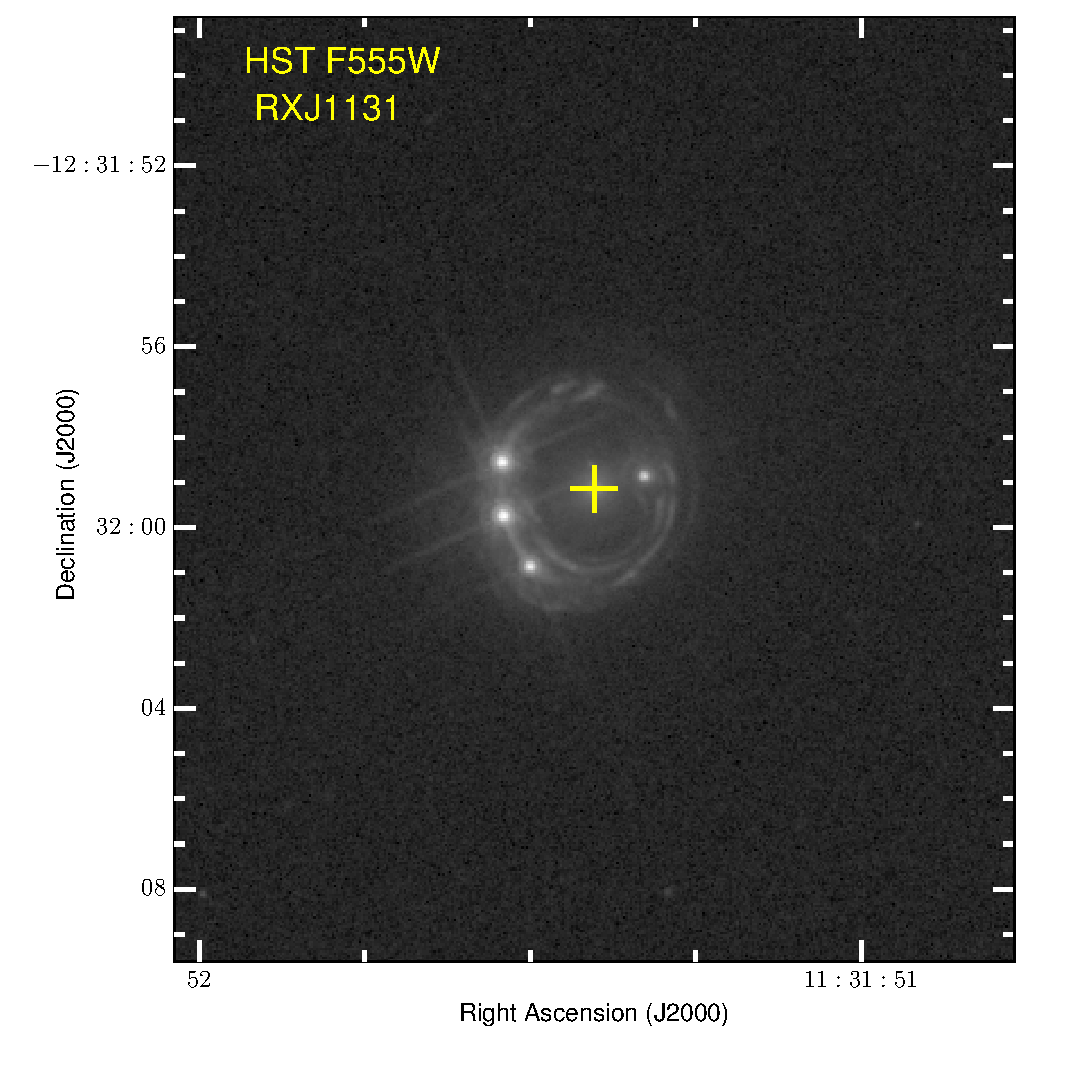
\includegraphics[scale=0.3]{Fig/F555W} &
\includegraphics[scale=0.37]{Fig/Manipulate_figsCROP}
\end{tabular}
\vspace{-1em}
\caption{ \fontsize{10pt}{12pt}\selectfont 
{
\textbf{RXJ1131-1231 stellar distribution and its reconstructed source plane
morphology}
{\em Left:} An optical image 
%obtained with the HST 
reveals the background AGN (knots)
and its host galaxy (arcs) with highly complex structures. The rest-frame UV emission (tracing
recent star formation) 
%in the background galaxy 
is lensed into an almost Einstein ring with radius $\sim$ 3.8". 
%The detection in rest-frame UV indicates recent star-formation.
{\em Right:} A lens modelling with the optical image identify an optically faint
companion (white; \citealt{Claeskens06a}), 
which we have recently confirmed with our dynamical lens model using \bco emission
(\Fig{model}) and is extremely dusty 
(\LIR$\sim$6$\times$10$^{12}$\Lsun) and gas-rich (\Fig{CO21mom0}; Leung \& Riechers, in prep.). 
A source plane reconstruction also shows seven spatially distinct components, 
highlighting the potential of our science target 
%is thus an excellent laboratory 
for studying the ISM conditions near starburst and AGN activities and offers an unparalleled
view into the early universe, with finer
detail than otherwise possible with current facilities. 
}
\label{fig:HST}}
\end{figure}

%\begin{figure}[!tbhp]
%\floatbox[{\capbeside\thisfloatsetup{capbesideposition={right,center},capbesidewidth=0.54\textwidth}}]{figure}[\FBwidth]
%{
%\vspace{-0.7em}
%\caption{ \fontsize{10pt}{12pt}\selectfont 
%{\textbf{RXJ1131-1231 stellar distribution and its reconstructed source plane
%morphology}
%{\em Left:} An optical image 
%%obtained with the HST 
%reveals the background AGN (knots)
%and its host galaxy (arcs) with highly complex structures. The rest-frame UV emission (tracing
%recent star formation) 
%%in the background galaxy 
%is lensed into an almost Einstein ring with radius $\sim$ 3.8". 
%%The detection in rest-frame UV indicates recent star-formation.
%{\em Right:} A lens modelling with the optical image identify an optically faint
%companion (white; \citealt{Claeskens06a}), 
%which we have recently confirmed with our dynamical lens model using \bco emission
%(\Fig{model}) and is extremely dusty 
%(\LIR$\sim$6$\times$10$^{12}$\Lsun) and gas-rich (\Fig{CO21mom0}; Leung \& Riechers, in prep.). 
%A source plane reconstruction also shows seven spatially distinct components, 
%highlighting the potential of our science target 
%%is thus an excellent laboratory 
%for studying the ISM conditions near starburst and AGN activities and offers an unparalleled
%view into the early universe, with finer
%detail than otherwise possible with current facilities. 
%}
%\label{fig:HST}}}
%{\begin{tabular}{@{}cc@{}}
%\hspace*{\fill}
%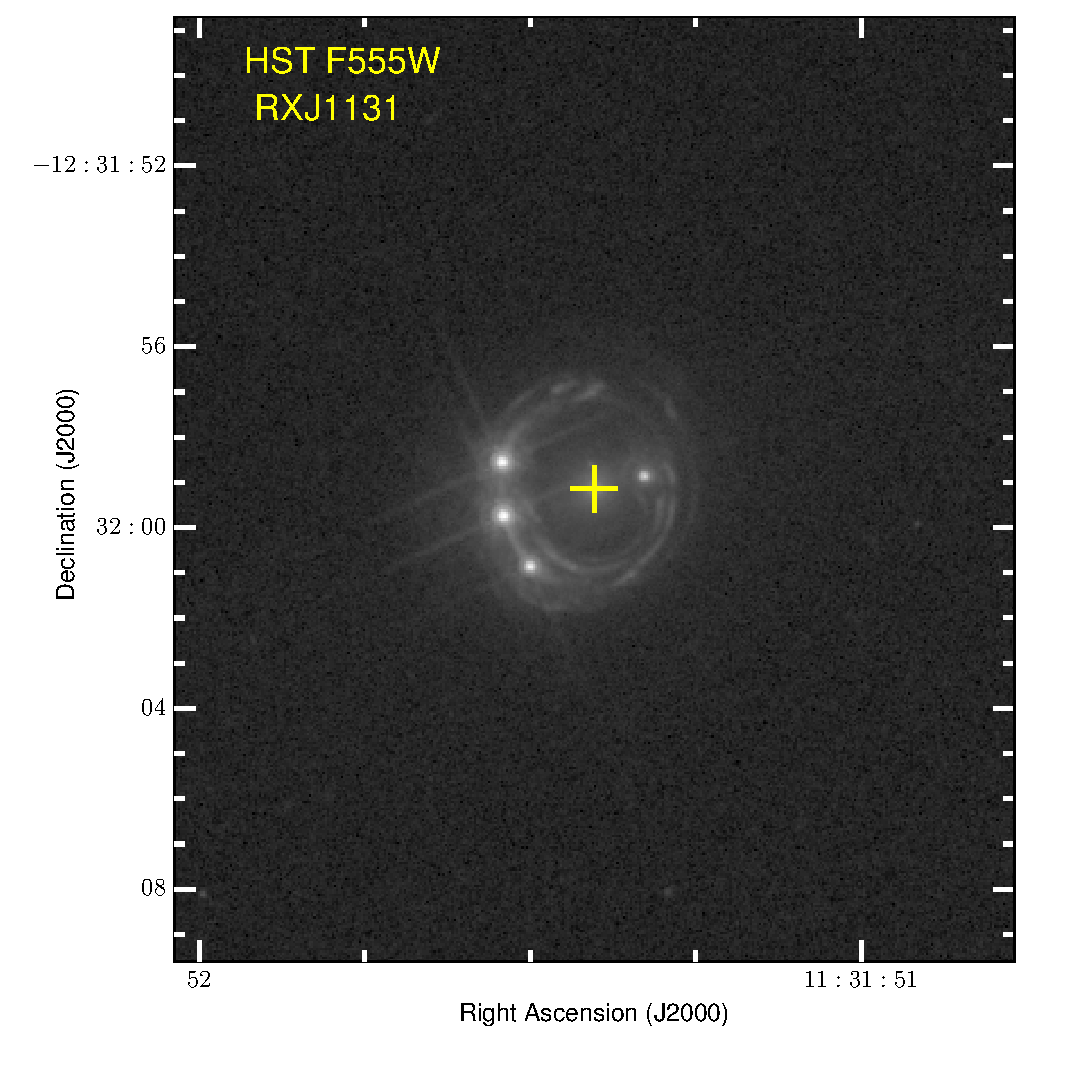
\includegraphics[scale=0.3]{Fig/F555W} \hfill % &
%\hspace*{-0.9em}
%\includegraphics[scale=0.35]{Fig/Manipulate_figsCROP}
%\hspace*{\fill}
%\end{tabular}}
%\vspace{-0.7em}
%\end{figure}

RXJ 1131-1231 is a quadruply imaged AGN with an Einstein Ring 
% of 3.8" in radius 
(\Fig{HST}). 
HST observations (rest-frame UV) have revealed distinct emission 
from recent star formation (arcs) and the AGN (knots) in the background galaxy \citep{Sluse03a},
demonstrating the complexity and the immense potential for probing the 
ISM conditions at astounding level of detail.
Lens modelling carried out with the optical images show
that the AGN resides in a star-forming region of $\sim$0.15" ($\sim$1 kpc)
in its host galaxy which is 1" across ($\sim$7 kpc), and identify
seven spatially distinct structures in the source plane of size 
$\sim$0.1" (\Fig{model}). Remarkably, emission originating from 
a spatially offset region from the AGN host galaxy has been identified 
at $\sim$ 2.4 kpc away, of $\sim$ 700 pc in size \citep{Brewer08a}, 
%in the source plane, 
indicating a nearby counterpart, which we have recently confirmed with
the \rot[CO]{2}{1} emission and our dynamical lens model, 
verifying the two host massive cool gas reservoirs and are at similar redshifts (\Fig{CO21mom0} \& \Fig{model}; Leung \& Riechers, in prep.). 
% The co-spatial CO emission with the optical emission (counter-arc)
% also confirms their massive cool gas reservoirs \Fig{CO21mom0}. 
Our SED modelling of the dust finds $L_{\rm IR}\sim6\times$10$^{12}$\Lsun 
(corrected for lensing). Hence, this target is a gas-rich ULIRG merger caught in the act. 

%%%%%%%%%%%%%%%%%%%%%%%%%%%%%%%%%%
% \section*{Proposed Observations and Immediate Objectives}
% \vspace{-0.25em}
\noindent {\bf Proposed Observations and Immediate Objectives}
We here propose to map (1): 
\eco at 0.15" resolution ($\sim$500pc in the source plane) and (2): \dhcn and \dhcop emission 
at 0.7" resolution (2.5 kpc). The 
%(high resolution) 
underlying continuum will addtionally provide
better constrain on the dust emission and distribution and thus surface density of the SFR. 
In conjunction with the large set of ancillary data obtained spanning from
rest-frame UV to radio and spectral line observations of \bco and \rot[CO]{3}{2}, our
proposed observations will address many questions in various aspects (see below).
The weak H$_2$O line falls in the same sideband as \eco, and thus our observations 
will as well provide constrains on the line strength and thus AGN feedback/excitation,
albeit the small number of detections at high redshift (R06?).

\underline{\bf Dynamics and kinematics:}

%\begin{figure}[!tbhp]
%\centering
%\includegraphics[scale=0.3]{../../Figures/CO_highOmom_CLIP5sigma}
%\vspace{-1em}
%\caption{ \fontsize{10pt}{12pt}\selectfont 
%{
%\textbf{RXJ1131-1231 kinematics and dynamics in \bco}
%{\em Left:} The observed velocity gradient is suggestive of a kinematically ordered disk. 
%% rotating with a maximum speed $v\sin i$ $\sim$ BLAH km/s.
%Limited by current spatial resolution, the intrinsic velocity gradient may
%be smaller than the beam size such that the smaller gradient are not 
%resolved, which may led to misinterpretation of the system to be 
%rotationally supported.
%{\em Right:} 2$^{nd}$ order moment map showing the velocity dispersion in the \bco emitting gas. 
%However, limited by the spatial resolution, beam smearing strongly decreases
%large-scale velocity gradients and increases observed dispersion.
%High resolution is thus necessary to distinguish the dichotomy between a rotating disk
%and mergers and/or the effect of a 
%companion on the internal dynamics of the AGN host galaxy.  
%This will enable us to understand the mechanisms driving the starburst and
%investigate whether dominant mode of star formation is like GMC in a stable disk or by fragmentation of
%dynamically unstable gas-rich disk. 
%% The proposed study will obtain data which will be complementary to the
%% HST data (rest-frame UV) which traces the stellar distribution. 
%}
%\label{fig:moments}
%}
%\end{figure}


\begin{figure}[!tbhp]
\floatbox[{\capbeside\thisfloatsetup{capbesideposition={right,center},capbesidewidth=0.6\textwidth}}]{figure}[\FBwidth]
{\hspace{-0.7em}
\caption{ \fontsize{10pt}{12pt}\selectfont {\textbf{RXJ1131-1231 kinematics and dynamics in \bco}
{\em Left:} The observed velocity gradient is suggestive of a kinematically ordered disk. 
Limited by current spatial resolution, the intrinsic velocity gradient may
be smaller than the beam size such that the smaller gradient are not 
resolved, which may led to misinterpretation of the system to be 
rotationally supported.
{\em Right:} 2$^{nd}$ order moment map showing the velocity dispersion in the \bco emitting gas. 
However, limited by the spatial resolution, beam smearing strongly decreases
large-scale velocity gradients and increases observed dispersion.
High resolution is thus necessary to distinguish the dichotomy between a rotating disk
and mergers and/or the effect of a 
companion on the internal dynamics of the AGN host galaxy.  
This will enable us to understand the mechanisms driving the starburst and
investigate whether dominant mode of star formation is like GMC in a stable disk or by fragmentation of
dynamically unstable gas-rich disk. 
% The proposed study will obtain data which will be complementary to the
% HST data (rest-frame UV) which traces the stellar distribution. 
}
\label{fig:moments}
}}
{\includegraphics[scale=0.3]{../../Figures/CO_highOmom_CLIP5sigma}}
\vspace{-0.7em}
\end{figure}


%\begin{figure}[tbph]
%\centering
%\includegraphics[width=0.45\textwidth]{Fig/olayCO21Spectra.eps}
%\caption{
%Overlay of spectra taken at different spatial positions along the greatest
%velocity gradient. 
%differential lensing of the different kinematic components of the galaxy
% \label{fig:CO21spectra}}
%\end{figure}

\begin{figure*}[tbph]
\centering
\includegraphics[width=0.37\textwidth]{Fig/olayCO21Spectra.eps}
\hspace{-0.45em}
\includegraphics[width=0.6\textwidth]{Fig/PostageStampModel.eps}
\caption{ \fontsize{10pt}{12pt}\selectfont {\textbf{Differential lensing with spatial variations and dynamical lens model}}
{\em Left:} Overlay of spectra taken at various spatial positions along the strongest velocity gradient, demonstrating 
differential lensing of the different kinematic components of the galaxy. Hence, higher resolution imaging of this source 
will allow us to probe the gas distribution.
{\em Right:} Velocity channels of the CO emission toward the gas-rich merger (red contours) overlaid on our best-fit 
lens model (grayscale). Clearly, there are spatial variations across different kinematic 
components, which is likely due to differential lensing. The foreground lensing galaxy is represented by a black dot, and 
the beam size is shown in the bottom right corner.
The velocity across the panels decreases from top left (red wing) to bottom right (blue wing), with $\Delta v\sim$100 \kms.
The reconstructed source morphology (magenta ellipse) is suggestive of a kinematically ordered galaxy. 
However, at the spatial resolution of our data, we cannot definitively infer its true morphology due to beam smearing. 
Higher-resolution imaging is needed to unambiguously determine the nature that gives rise to the observed velocity gradient. The proposal observations will confirm if the system is rotationally supported or highly turbulent (due to AGN or tidally disrupted if merging with the companion). 
\label{fig:model}}
\end{figure*}

% Gas distribution 
The CO emission shows an asymmetric double-horned line profile (\Fig{CO21mom0}), which 
indicates the effect of differential lensing and that the cool gas is spatially distributed (\Fig{model}). 
Hence, our proposed observations will probe the spatial variations of the molecular gas. 
% gas kinematics
The 1$^{\rm st}$ moment map (\Fig{moments}) and the velocity gradient 
across the source plane (Fig.~\ref{fig:model}) in our model suggests
that our source is kinematically ordered (reminiscent of a rotating disk). Yet,  
the spatial resolution of this data is insufficient to infer the true 
kinematics due to beam smearing. Besides, 
% velocity dispersion suggest the source may be dispersion dominated (\Fig{moments}). 
an unusually high velocity dispersion 
$\gtrsim$400\kms at the central region(\Fig{moments})  hint at 
%plausible 
perturbations from the central AGN and/or
internal turbulent motion due to interactions with the companion
and/or instability due to the huge gas reservoir.
Higher-resolution imaging is absolutely necessary to 
%map the intrinsic velocity gradient and dispersion in order 
to unambiguously determine the nature that gives rise to 
the observed velocity gradient and 
confirm if the galaxy is disk-like but disrupted or merging
and whether it is dominated by internal random 
motions (in addition to large-scale orbital velocity, if confirmed to be disk-like in 1st moment map)
to distinguish the major mechanism driving the starburst: merger-driven 
versus gas-rich clumpy disk, which show similar velocity profile in low-resolution data. 

We also aim to spatially separate/resolve the kinematic 
signatures of the gas clumps in the AGN host galaxy to probe
the kinematical and dynamical state of the gas, and 
how the gas distribution is affected. 
At the proposed resolutions, we will also
obtain a better-constrained dynamical lens model
and be able to probe the gas in the kinematically related companion 
and its internal dynamics. 
The proposed observations will also highly complementary to optical image,
% spider diagram in the iso-velocity contours
allowing a comparison between the gas and stellar distribution.
% probing the dynamics of the excited-gas in a high-z source at resolution 
% otherwise impossible.

\underline{\bf Physical properties and dense gas line ratio maps:}
% Between HCN/HCO+:
Since the critical densities of HCN rotational transitions are $\sim$5 times
higher than \hcop, they trace different gas phases.
% with different densities. 
The line fluxes and spatially resolved line ratio maps will thus enable us 
 to constrain the density and temperature of the molecular gas around 
 the AGN, its star-forming host galaxy, and in its companion, providing perceptive clues to how these
activities and galaxy interactions alter the chemical composition of the ISM/ISM chemistry (e.g. HCN 
and \hcop enhancements in different regions), and thus the evolution these ubiquitous dusty mergers.
Due to the difference in abundances and excitation conditions of these molecules,
\dhcn/\dhcop can be used to separate activities/emission originating from AGN or starburst
\citep{Imanishi10, Izumi13a}, % \citep{Imanishi14a}.
which sheds light on AGN and star-formation feedbacks and clues to interpret 
the evolutionary stage of the galaxy (Baan+08).

% e.g. HCO+/HCN is found to be enhanced in star-forming regions 
% (in PDRs, SN shocks [can enhance HCO+]; Maijerink+07). 
% Thus the line ratio may be diagnostic to distinguish between XDRs, PDRs or 
% deeply embedded star-formation (Blake+87;  Bayet+08); 
% where lower ratio may suggest low-density XDR or dense PDRs (Costagliola+11).
% this assumes line ratios are directly linked to relative abundances 
% (Krips+08; then spatially resolved line ratio traces abundance gradient)
% but may not be true for HCN and HCO+.

\underline{\bf Excitation conditions:}
% between CO/HCN
The line ratio \comol(low-J)/HCN probes the dense gas fraction, abundance, and excitation. Thus, we will 
map out the spatial variations and gradients in the physical conditions of
the gas within the galaxies, providing extra constraints on the star-formation activity.

We will combine these data [tracing the excited emission] with our existing lower-J CO 
data to diagnose the excitation conditions and the heating source of the gas. [Since the high-density tracers probe 
the star-forming molecular dense gas regions and
the low-density tracers probe the relatively unperturbed larger-scale molecular
environment.]

% Some high excitation CO SLEDs are found in local ULIRGs, suggesting strong
% supersonic turbulence and cosmic ray rather than UV photons from SF sites as heating source, 
% warming up the large amounts of dense gas in these SBs.
% Thus we will be able to extract the physical and dynamical states of the ISM environment.

\underline{\bf Star-formation Law:}
Our proposed observations will furnish data to carry comparative studies
between the \LIR, SFR$_{\rm IR}$, SFR$_{\rm UV}$, surface densities of SFR, CO, HCN and \hcop,
providing stringent constraints on the relation between molecular gas and star-formation on sub-kpc scales and on the mechanisms driving the mammoth SFR at earlier epochs, giving rise to the observed stellar-assembly history.

%%%%%%%%%%%%%%%%%%%%%%%%%%%%%%
% closing
% mechanisms and physical processes and on different scales.
\par 
Our proposed observations therefore provide an exceptional opportunity to investigate
the physical properties and dynamical structures of different gas phases in the ISM of mergers 
and distant galaxies with exquisite details.
These are vital to improve our current understanding 
on the star-formation processes at the cosmic epoch 
where the contribution of dusty, star-forming galaxies to the cosmic SFR density is steeply rising 
\citep{LeFloch05a}. 
This will also provide a benchmark in utilizing high-dipole moment molecules as 
routine tracers to study star-formation in relatively poorly-studied high-z populations
and demonstrate the capabilities of ALMA in mapping these much fainter emission in distant galaxies.
 The proposed observations with our science target will therefore provide a giant leap on 
our understanding -- putting high-z systems into the context of nearby studies and lay the groundwork to 
routinely perform such studies at higher redshifts in the ALMA full operations cycle in the near future.

%%%%%%%%%%%%%%%%%%%%%%%%%%%%%%%%%%
%\section*{Technical overview}
%\vspace{-0.25em}
%{\bf Technical overview}
%We propose to image the gravitationally lensed merger at z$\sim$0.65 in the redshifted  
%{\bf (1)} \eco line at $\sim$0.15" resolution (array config. C40-5) 
%and {\bf (2)} \dhcn and \dhcop at $\sim$0.7" resolution (C40-3). 
%We assume a line width (FWHM) of 700\kms based on our \bco observations 
%(\Fig{CO21mom0}) for both science goals and the source size from our dynamical lens model, which
%takes into account the asymmetric line emission
%and spatial extent due to differential lensing. 
%We thus expect the source to be resolved over 153 beams 
%and 7 beams at 0.15" and 0.7", respectively. 
%We compute target sensitivity for \eco using \bco line flux and adopt a conservative 
%line ratios between \aco and \bco, and \eco based on SMGs \citep{CW13}. 
%We compute expected sensitivity for \dhcn from \aco using a conservative line ratio
%between \aco and \ahcn and \dhcn based on (U)LIRGs (GS04; P07).
%We estimate a line flux for \dhcop based on the line ratio \dhcn/\dhcop found in ULIRGs 
%\citep{Greve09a}. We use the most stringent sensitivity estimates 
%among \dhcn and \dhcop as our sensitivity goal. The latter sets the overall requirement. 
%To secure enough S/N for our model, 
%we require a minimum of 8$\sigma$ of 0.47 mJy beam\pmOne and 0.07 mJy beam\pmOne
%per 150 \kms channel to reconstruct the dynamical structure in the source plane for the science goals, respectively. 
%We therefore request a total time of 7.0 hours to complete our science goals. 

%%%%%%%%%%%%%%%%%%%%%%%%%%%%%%%%%%
%\section*{Potential for publicity}
%\vspace{-0.25em}
{\bf Potential for publicity} 
I will publish a paper on this if I get the data I need. SOME TEXT
The proposed observations will serve as a demonstrative case
of the dense, excited gas in high-z galaxies at high resolution. 
high potential for publicity. 
% This will enable us to demonstrate galaxies in this epoch, blah beyond capabilities of 
% current facilities. 


\begin{figure*}[tbph]
\centering
% \includegraphics[width=0.25\textwidth]{Fig/{F555WCO21_mom0_single.invertedgray}.eps}
\hspace*{\fill}
\includegraphics[width=0.25\textwidth]{Fig/F555W_REDCentBLUE.png}
\hspace*{-0.9em}
\includegraphics[width=0.45\textwidth]{Fig/SpecCO21_twinx.eps}
\hspace*{\fill}
\caption{ \fontsize{10pt}{12pt}\selectfont {\textbf{Detection of a gas-rich merger with spatial variations traced by \bco}
{\em Left:} The (red, green, blue) contours correspond to the velocity-integrated line flux of different velocity channels (red wing, line center, blue wing) in our \rot[CO]{2}{1} data. 
Strikingly, the spatially-resolved molecular gas emission shows a different lensing configuration 
than in the optical.
The counter-arc structure as shown by the red wing and its redshift (see right) is evident of a gas-rich source. This companion galaxy is consistent with the dusty source discovered with {\it Herschel}, 
which is faint in the optical as expected (the white component in Fig.~\ref{fig:HST}).
% \fontsize{10pt}{12pt}\selectfont {\textbf{PdBI \rot[CO]{2}{1} dynamically resolved line profile} 
{\em Right:}
The continuum-subtracted spectrum shows a double-horned profile, where the red wing is significantly brighter. Our lens modelling suggests that this arises due to differential lensing across the 
kinematic components of the source.
% As indicated on the top axis, 0 km/s corresponds to z=0.655. 
Our proposed observations will allow us to investigate the fuel and mechanisms responsible for the intense star-formation in the AGN host galaxy. We here aim to spatially and dynamically resolve the dense, excited gas emission, which will allow us to unambiguously examine the dynamic structure of the ISM in the distant merger and provide observational constants on the star-formation and stellar-assembly history at the epoch where the SFR density is steeply rising across cosmic times.
}
 \label{fig:CO21mom0}}
\end{figure*}


\noindent \bf {References}
{\fontsize{10pt}{12pt}\selectfont
	\bibliography{RXJ_ALMAC4}
}

\end{document}
